\setcounter{section}{62}
\section{Количество чисел на отрезке, значения которых лежат в отрезке: решение с деревом отрезков деревьев поиска.}
\par \textbf{Формулировка задачи:} Дан статический массив $a_0, \ldots, a_n$. Поступают запросы "найти количество чисел на отрезке $[l,r]$, значения которых лежат в пределах $[x,y]$". Можем свести эту задачу к следующей: найти количество чисел из $[l.r]$, которые $\leqslant y$, и потом вычесть результаты для $y$ и $x-1$.
\par \textbf{Идея:} Строим дерево отрезков на массиве, в каждой вершине которого хранится дерево поиска на элементах контролируемого подотрезка. В дереве поиска мы умеем отвечать на запрос "количество элементов $\leqslant y$": в каждой вершине храним количество элементов в поддереве и просто находим, какой порядковой статистикой является $y$. Тогда для выполнения нашего запроса нужно будет просуммировать результаты, полученные из деревьев поиска, на всех подотрезках.
\begin{figure}[h]
    \centering
    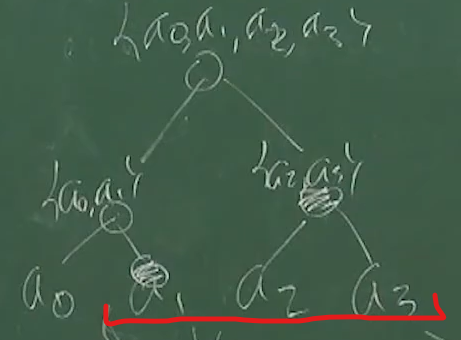
\includegraphics[scale=0.8]{images/63-64_dodd}
    \caption{Ответ на запрос на отрезке $[1,3]$}
\end{figure}
\par \textbf{Асимптотика:} Как мы уже доказывали для дерева отрезков, для ответа на один запрос мы посещаем логарифмическое количество вершин. В каждой вершине мы должны сделать запрос в дерево поиска (асимптотика: $O(\log n)$). Таким образом, общая асимптотика ответа на запрос: $O(\log^2 n)$
\\
\\
\\
\\
\\
\\
\\
\\
\\
\\
\\
\setcounter{section}{63}
\section{Количество чисел на отрезке, значения которых лежат в отрезке: Fractional Cascading.}
\par \textbf{Идея:} Строим "дерево MergeSort": для каждого подотрезка храним отсортированный массив его элементов. Кроме того, для каждого элемента $x$ массива храним два числа: индексы наибольших элементов в наследниках, которые $\leqslant x$.
\begin{figure}[h]
    \centering
    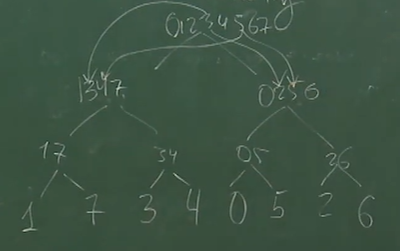
\includegraphics{images/63-64_fractional cascading}
    \caption{Пример дерева}
\end{figure}
\par Таким образом для ответа на запрос нам необходимо \begin{enumerate}
    \item С помощью бинарного поиска найти число $y$ в массиве из корневой вершины
    \item Спускаться как в обычном дереве отрезков, но "по стрелкам"
    \item Просуммировать все индексы, в которых мы остановились (именно столько чисел $\leqslant y$ будет в каждом из отрезков).
\end{enumerate}
\par \textbf{Асимптотика:} $O(\log n)$ на бинарный поиск + $O(\log n)$ на спуск в дереве отрезков $\Rightarrow$ общая асимптотика: $O(\log n)$